\subsection{Budget constraint}

In order to attract FDI, the government official offers foreign firms with benefits such as market size or cheap labor. These resources are finite, thus imposing a budget constraint on the FDI that the official can attract.

When considering a FDI project, the government official decides between two benefits that the project may bring, i.e. technological spillover and private benefits. While there are other benefits to FDI, such as employment generation and capital, technological spillover is crucial to the improvement in total factor productivity, an ingredient of economic growth. Private benefits of FDI to government officials can be either illegal (e.g. bribes) or legal (e.g. informal network with foreign firms that leads to contracts for friends and families, campaign finance contribution).
 
There is a trade-off between these two benefits. To encourage technological spillover, governments frequently impose conditions on foreign firms, such as forming a joint venture or local content requirement. These requirements constrain the ability of firms to use their physical and management capital optimally, reducing the efficiency and thus profitability of firms. Similarly, when firms are forced to offer private benefits to officials (e.g. bribes, contracts with officials' relatives), it introduces both an upfront cost as well as the cost of uncertainty (as these private benefits are informal and not encoded transparently). Therefore, offering officials private benefits also reduces the profitability of firms. Given that firms themselves have to maintain a minimum amount of profitability (akin to reservation wage), when they offer one type of benefits they would have to reduce the others. Therefore, if the government official demands one type of benefit, they will get less of the other. In this way, technological spillover and private benefits are two separate goods that the officials have to choose given the budget constraint that they have to attract FDI.

(Basically the ``budget'' comes from the fact that the country's endowment is turn into profit to the firm. When the firm makes profit, it can use part of that profit to pay for either private benefits of technological spillover.)

The location of the budget constraint depends on the endowment of the official. The better endowment the official has, the budget constraint shifts to the right, meaning that he will be able to get both more technological spillover and more private benefits. For example, in \Cref{fig:budget_constraint}, the official with more endowment has the budget constraint on the right. As we can see, he is capable of attaining the $(s_2, b_2)$ bundle, with both $s_2 > s_1$ and $b_2 > b_1$.

\begin{figure}[!ht]
	\centering
    
\includegraphics[width=0.75\textwidth, height=0.75\textheight,keepaspectratio]{../figure/budget_constraint}
    \caption{Budget constraint}
    \label{fig:budget_constraint}
\end{figure}

\subsection{Relative price (slope of the budget constraint)}

The intercepts of the budget constraint is determined by the ``price'' of the two goods, i.e. how easily the official can obtain technological spillover and private benefit from the foreign investors.

The ``price'' of technological spillover would be the absorptive capacity of the local economy, which I argue to be the presence of private firms that are able to absorb technology from foreign firms. This absorption can happen via two channels. First, private firms enter into the supply chain of the foreign firms, thus subject to higher standards of foreign firms and can also imitate the foreign firms' management techniques via exposure. Second, local employees employed by foreign firms may learn from the experience in the foreign firms and take that knowledge when they transfer to local firms. This channel also requires the presence of private firms that are able to compete with foreign firms for these high quality labor.

The ``price'' of private benefit would be how easily the government officials can extract these benefits from the foreign firms. This parameter would capture real world elements such as the background of the firm. For example, firms that come from countries where corruption is more prominent or accepted would have a higher propensity to bribe. Or if firms come from countries who have signed onto the OECD anti bribery conventions would be more hesitant to bribe, given the punishment that they may face from their home governments for bribing.

Together, these two prices determine the slope of the budget constraint. See \Cref{fig:relative_price}

\begin{figure}[!ht]
	\centering
    \includegraphics[width=\textwidth, height=\textheight,keepaspectratio]{../figure/absorptive_capacity}
    \caption{Relative price of spillover and rent}
    \label{fig:relative_price}
\end{figure}

\subsection{Indifference curve}

The official has a convex indifference curve, meaning that there is decreasing marginal utility to both spillover and private benefit. This assumption is standard and makes intuitive sense. As the official accumulates more and more private benefit, there are fewer and fewer things to spend them on, his consumption is satiated and produces less utility. Similarly, when more and more technological spillover happens, it becomes less of a bottleneck to the economy, thus voters (or higher-ups) may be come less concerned, and it brings less electoral (or promotional) benefits.

The shape of the indifference curve denotes the relative weight the official assigns to the two goods, spillover and private benefit. When the curve is steep, it means that the official is willing to trade a lot of spillover for a small increase in private benefit. Vice versa, a flatter curve indicates that the official values spillover more.

Politically, the steepness of the indifference curve depends on the time horizon of the official. This is because technological spillover takes time to happen and leads to increase in economic growth, whereas private benefit is immediate. The longer time horizon does the official have, the more heavily does he weigh technological spillover effect. In \Cref{fig:indifference_curve}, the blue indifference is flatter and signifies more weight assigned to spillover effect. As we can see, the official does choose a bundle that has more spillover effect than private benefits.

\begin{figure}[!ht]
	\centering
    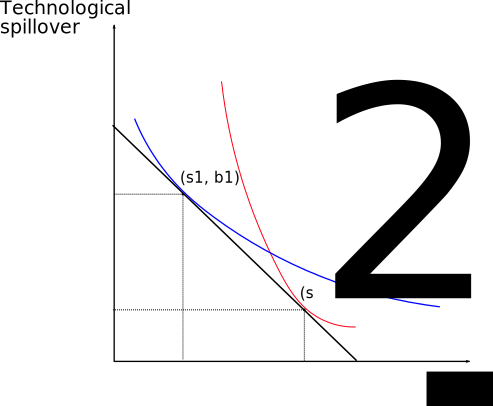
\includegraphics[width=0.75\textwidth, height=0.75\textheight,keepaspectratio]{../figure/indifference_curve}
    \caption{Time horizon and the shape of the indifference curve}
    \label{fig:indifference_curve}
\end{figure}

What affects this time horizon? Term limits, the stability of the regime, the probability of electoral success.

\subsection{Implication}